%!TEX root = /home/renaud/Documents/EPL/tfe/latex/tfe.tex
\section{The bi-overturner class of problems}
The bi-overturner problems basically consist of two \textit{overturner} circulations models side-by-side, hence the name. However, although the overturner circulation was initially developed as an idealization of the meridional circulation in the Atlantic ocean, bi-overturner problems do not model any "real-life" problem. Therefore, the values of the different physical parameters are given without justification, although most of the quantities are inspired from the values proposed in \cite{timmermans2006masterthesis}. The bi-overturner problems are really used as a mathematical tool to test the method, and using the overturner circulation ensures that the velocity field that we consider satisfies the continuity equation and no-through boundary condition everywhere on $\partial \Omega$. The domain that we consider is $\Omega = [-L,\,L]\times[0,\,H]$. Let $\Omega^- = [-L,\,0[\times[0,\,H]$ and $\Omega^+ =\; ]0,\,L]\times[0,\,H]$. If $\psi(y,z;y_0,z_0)$ denote the streamfunction defined in~\eqref{eq:psi_overturner} with parameters $y_0 \in\; ]0,\,L[$ and $z_0 \in\; ]0,\,H[$, then the streamfunction $\varphi$ of the bi-overturner problems is defined as
\begin{equation} \label{eq:psi_2box}
	\varphi(y,z) = \left\{ 
		\begin{array}{lrr}
			\psi(L+y,z;y_0,z_0) & \mbox{if} & (y,z) \in \Omega^-,\\
			0 & \mbox{if} & (y,z) \in \{(0,z)\;|\;z \in [0,\,H]\},\\
			-\psi(y,z;L-y_0,z_0) & \mbox{if} & (y,z) \in \Omega^+,\\
		\end{array}
	\right.
\end{equation}
The streamfunction $\varphi$ has two extrema of equal strengths: a maximum at $(y_0^-,z_0)$ with $y_0^- := -L+y_0 = -y_0^-$ and a minimum at $(y_0^+,z_0)$ with $y_0^+ := L-y_0$. The overturner-like circulation is clockwise in $\Omega^-$ and counterclockwise in $\Omega^+$. The horizontal and vertical velocities $v$ and $w$ are given by
\begin{equation} \label{eq:u-psi_2box}
	v = -\frac{\partial \varphi}{\partial z}, \quad w = \frac{\partial  \varphi}{\partial y}.
\end{equation}
 Isolines are shown in figures~\ref{fig:v2box} and~\ref{fig:w2box} respectively. The key feature is that $v(0,z) = 0$, namely the horizontal velocity is zero on the whole segment $y = 0$. Hence, if there is no horizontal diffusion, a passive tracer's particle starting in $\Omega^-$ can never reach $\Omega^+$ and conversely. In that case, we can imagine that there is a vertical wall implying no-through boundary conditions at $y=0$ and the graph is not ergodic. But if the horizontal diffusivity is nonzero in some area near $y=0$, then exchange of particles between $\Omega^-$ and $\Omega^+$ can happen in that area. Now we suppose that the diffusivity tensor $\b K$ is diagonal:
 \begin{equation}
 	\b K(y,z) = \begin{pmatrix} K_{yy}(y,z) & 0\\ 0 & K_{zz} \end{pmatrix}.  	
 \end{equation} 
We assume that the vertical diffusivity $K_{zz}$ is constant and equal to $10^{-3}$ [$\rm{m^2/s}$]. Now we introduce the parameter $\alpha \in [0,1]$ and define $z^* = \alpha H$. We choose an horizontal diffusivity $K_{yy}$ of the form
\begin{equation} \label{eq:Kh2box}
	K_{yy}(y,z) = \begin{cases}
			10^4\ \rm{[m^2/s]} & \mbox{if} \quad y_0^- \le y \le y_0^+ \quad \mbox{and} \quad z^* \le z \le H,\\
			10^3\ \rm{[m^2/s]} & \mbox{if} \quad -L \le y < y_0^- \quad \mbox{or} \quad y_0^+ < y \le L,\\
			0\ \rm{[m^2/s]}  & \mbox{otherwise}.
		\end{cases}
\end{equation}
Now, exchange between $\Omega^-$ and $\Omega^+$ is possible but only above $z^*$.\footnote{From a numerical, random-walk, point of view, we should also ensure that $y_0^+ = |y_0^-|$ is sufficiently large. If not, it would be numerically possible for particles lying below $z^*$ and before $y_0^-$ (resp. after $y_0^+$) to jump from $\Omega^-$ (resp. $\Omega^+$) to $\Omega^+$ (resp. $\Omega^-$).} Hence, we can imagine that there is a vertical, no-through wall of height $z^*$ at $y=0$. The situation is depicted on figure~\ref{fig:Kh2box}. For the next, we call \textit{exchange zone} the area where $K_{zz} = 10^4$ $\rm{[m^2/s]}$ (dark gray zone in figure~\ref{fig:Kh2box}). Making $\alpha$ vary between $0$ and $1$ defines a class of bi-overturner problem where the vertical wall's height $z^*$ at $y=0$ vary between $0$ and $H$. Two examples of trajectories with the same initial condition are shown for $\alpha = 0.75$ in figures~\ref{fig:withouttransfer} and~\ref{fig:withtransfer}.

\begin{figure}[!htp]
	\centering
	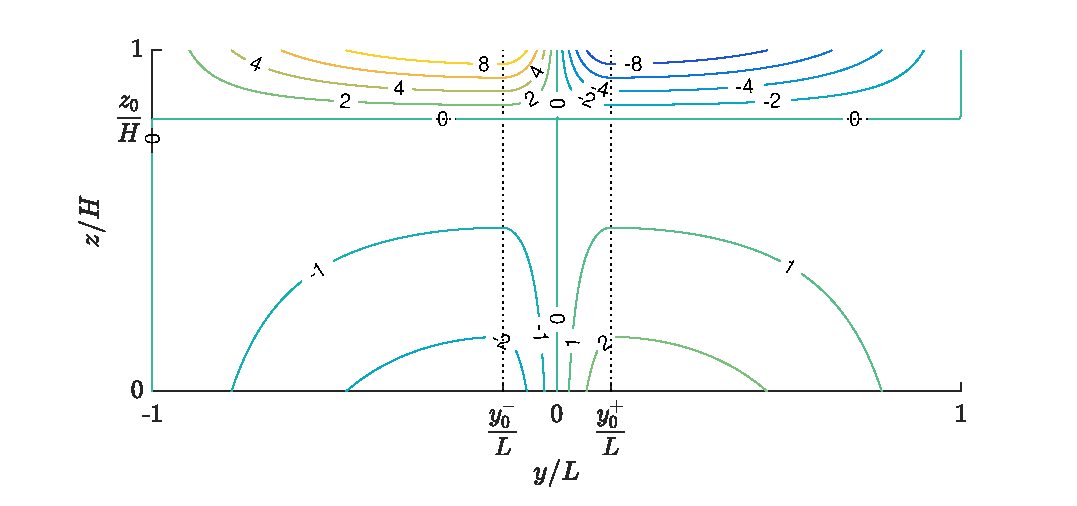
\includegraphics[width=\textwidth]{fig/problem2box/v2box_timmermans.eps}
	\caption{Isolines of the horizontal velocity $v$ for bi-overturner problems.}
	\label{fig:v2box}
\end{figure}

\begin{figure}[!htp]
	\centering
	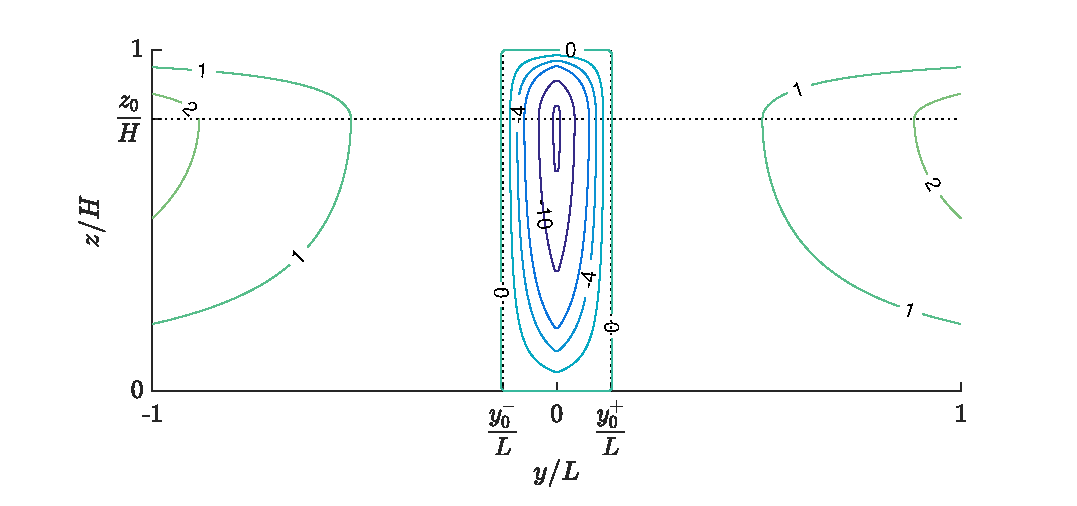
\includegraphics[width=\textwidth]{fig/problem2box/w2box_timmermans.eps}
	\caption{Isolines of the horizontal velocity $w$ for bi-overturner problems.}
	\label{fig:w2box}
\end{figure}

\begin{figure}[!htp]
	\centering
	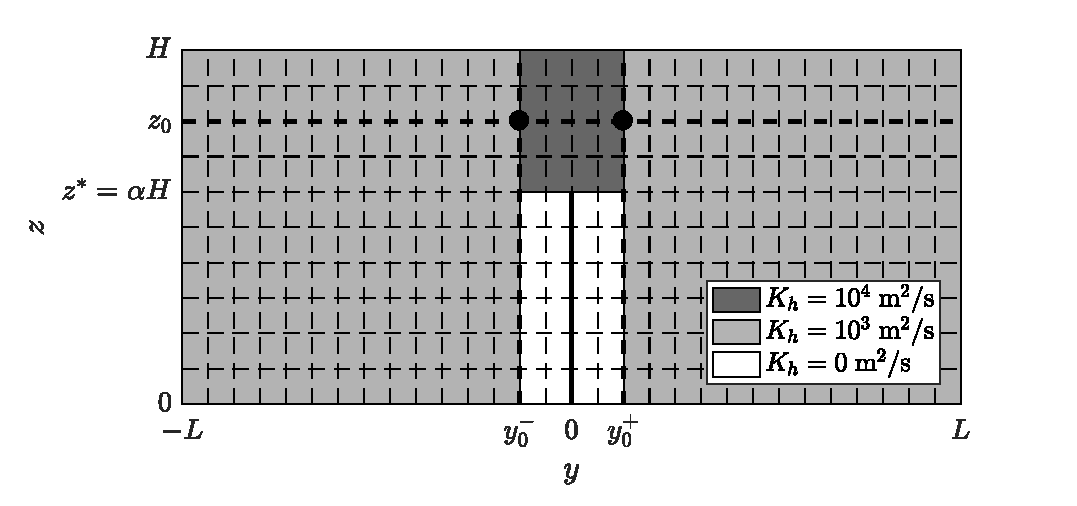
\includegraphics[width=\textwidth]{fig/problem2box/problem.eps}
	\caption{Illustration of the decomposition of the domain into boxes corresponding to the nodes of the directed graph. The values of $K_{yy}$ are also shown for $\alpha = 0.6$, and the fictitious wall is represented by the black continuous line. Here the particle enters the exchange zone but finally stays in $\Omega^-$.}
	\label{fig:Kh2box}
\end{figure}

\begin{figure}[!htp]
	\centering
	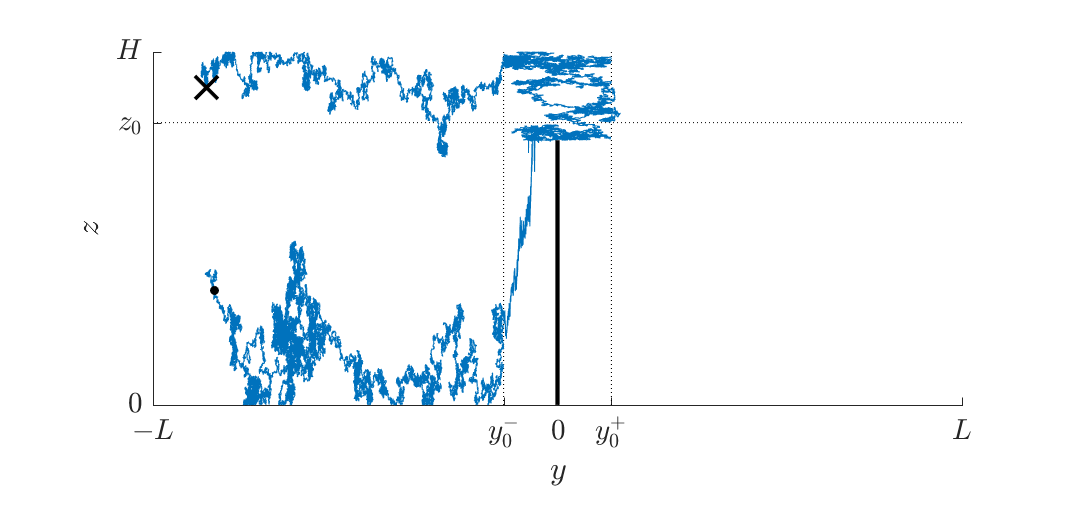
\includegraphics[width=\textwidth]{fig/problem2box/traj_without_transfer5.eps}
	\caption{Example of a particle trajectory in the bi-overturner model with $\alpha = 0.75$. The black cross represents the initial position whereas the black dot shows the final position. The simulation time is 200 years.}
	\label{fig:withouttransfer}
\end{figure}

\begin{figure}[!htp]
	\centering
	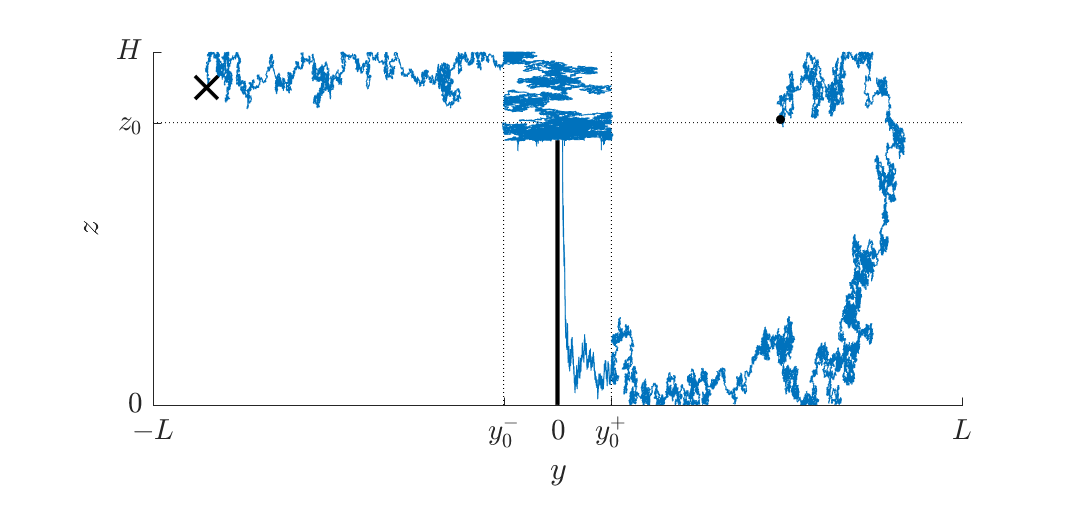
\includegraphics[width=\textwidth]{fig/problem2box/traj_with_transfer2.eps}
	\caption{Example of a particle trajectory in the bi-overturner model with $\alpha = 0.75$. The black cross represents the initial position whereas the black dot shows the final position. The simulation time is 200 years.}
	\label{fig:withtransfer}
\end{figure}
When $\alpha = 1$, the obvious compartmental model is made of the two compartments $\Omega^-$ and $\Omega^+$ which do not communicate with each other. Suppose that different amounts of passive tracer are released into $\Omega^-$ and $\Omega^+$ at a given time; the concentration in each compartment tends to become uniform in time due to diffusion, but the concentration in $\Omega^-$ depends only on the initial quantity of tracer released in $\Omega^-$ and similarly for the concentration in $\Omega^+$. At the contrary, when $\alpha = 0$ the concentration tends to become uniform over the whole domain when time goes to infinity. Hence, we can expect three types of partitioning to be dominant at different time scales: a three-communities partitioning with left and right compartments and an exchange zone in between; a two-communities partitioning corresponding to $\Omega^-$ and $\Omega^+$; and finally a trivial partitioning with one single community for very long time scales. For intermediate values of $\alpha$, we expect a behavior similar to the case $\alpha = 0$ when $\alpha$ is close to $0$. When $\alpha$ is close to $1$ but still different from $1$, exchange can still happen between $\Omega^-$ and $\Omega^+$. However, in terms of communities, we expect the two-community partitioning to be dominant for long time scales.  

\subsection{Application of the stability method}
The partitioning results are presented here for $\alpha = 1$, $\alpha = 0.75$, $\alpha = 0.5$, $\alpha = 0.25$ and $\alpha = 0$. For every value of $\alpha$, the transition probability matrix is computed at $T = 1$ year on a discretization like the one presented in figure~\ref{fig:Kh2box}, namely with $\nby = 30$ and $\nbz = 10$. $P_0 = 10\,000$ particles are initially released in every grid cell. The stability software is run using a vector of Markov times taking values between $10$ and $10^3$. Since we have computed the transition probability matrix for $T = 1$ year, one unit of Markov time correspond here to one year. Notice that in the case where $\alpha = 1$, the graph is not ergodic (it is composed of two ergodic classes) and a random teleportation probability \mtlb{tau} $= 10^{-3}$ is used when running the stability software. When $\alpha < 1$, \mtlb{tau} $=0$ is used.
The stability, number of communities and variation of information curves are shown in figures~\ref{fig:staba1}, \ref{fig:staba75}, \ref{fig:staba5}, \ref{fig:staba25} and~\ref{fig:staba0} for the different values of $\alpha$. Most robust communities correspond to plateaux in the community curve together with a low variation of information. Whatever the value of $\alpha$, the number of communities goes to $2$ after maximum $50$ years, and the corresponding variation of information is almost zero. In every case, the two-communities partitioning corresponds as expected to $\Omega^-$ and $\Omega^+$. It is shown in figure~\ref{fig:cluster_a25_2} for the case $\alpha = 0.25$. In that case, the boundary is perfectly straight: this corresponds to the intuition and it is conform to the remark made on page \pageref{remark:straightboundaries}. In some other cases, like when $\alpha = 0.5$, the boundary is not exactly a straight line. The situation is depicted in figure~\ref{fig:cluster_a5_2}. However, we have to remember that neither the transition probability matrix nor the stability partitioning is solved exactly. Hence, we can consider that the irregularity in the boundary of the communities is due to those numerical artifacts: if a box model has to be build from the partitioning shown in figure~\ref{fig:cluster_a5_2}, the compartments should of course be chosen with a vertical boundary. This illustrates the fact that when using a community-detection algorithm to build compartments for a box model, the communities should not be blindly interpreted as being the relevant compartments. In particular, if the boundaries of the communities are almost but not exactly vertical and horizontal, one should consider straight boundaries for the compartments. Community detection should thus be considered as a guide towards choosing relevant compartments, rather than as a method providing the exact perfect compartments.

When $\alpha = 0.75$, a small three-communities plateau starts appearing around 40 years, just before the two-communities plateau. This plateau grows as $\alpha$ decreases. The corresponding clusterings are shown in figures~\ref{fig:cluster_a25_3} and~\ref{fig:cluster_a0_3}, where a community corresponding to the exchange zone appears, as expected.

In figure~\ref{fig:staba0} corresponding to the case $\alpha = 0$, peaks corresponding to oscillations between two and three communities are observed around 300 and 400 years. As stated in chapter~\ref{chap:clustering}, the number of communities should decrease with time, and those oscillations are thus due to the fact that the stability partitioning is only solved approximately. However, this shows that the two- and three-communities clusterings have similar stabilities at those times. Finally, remember that we expected to find a single-community partitioning for very long Markov times in the case $\alpha = 0$, which does not appear here. Such a clustering would probably appear if we run the stability software for longer Markov times.

% Hopefully this introductory example shows how a community-detection algorithm could be use to build compartment models, and provide intuition about why it could work. The communities found depend on the time scale considered but this is not a problem since it could also be the case for the compartments. Notice that we do not to build compartmental models for the bi-overturner class of problems because the compartments are obvious in this case, and it is thus not the goal of this section. In the next section, the method is applied on the overturner problem and we should try to build a compartmental model for that problem. 

\begin{figure}[!htp]
	\centering
	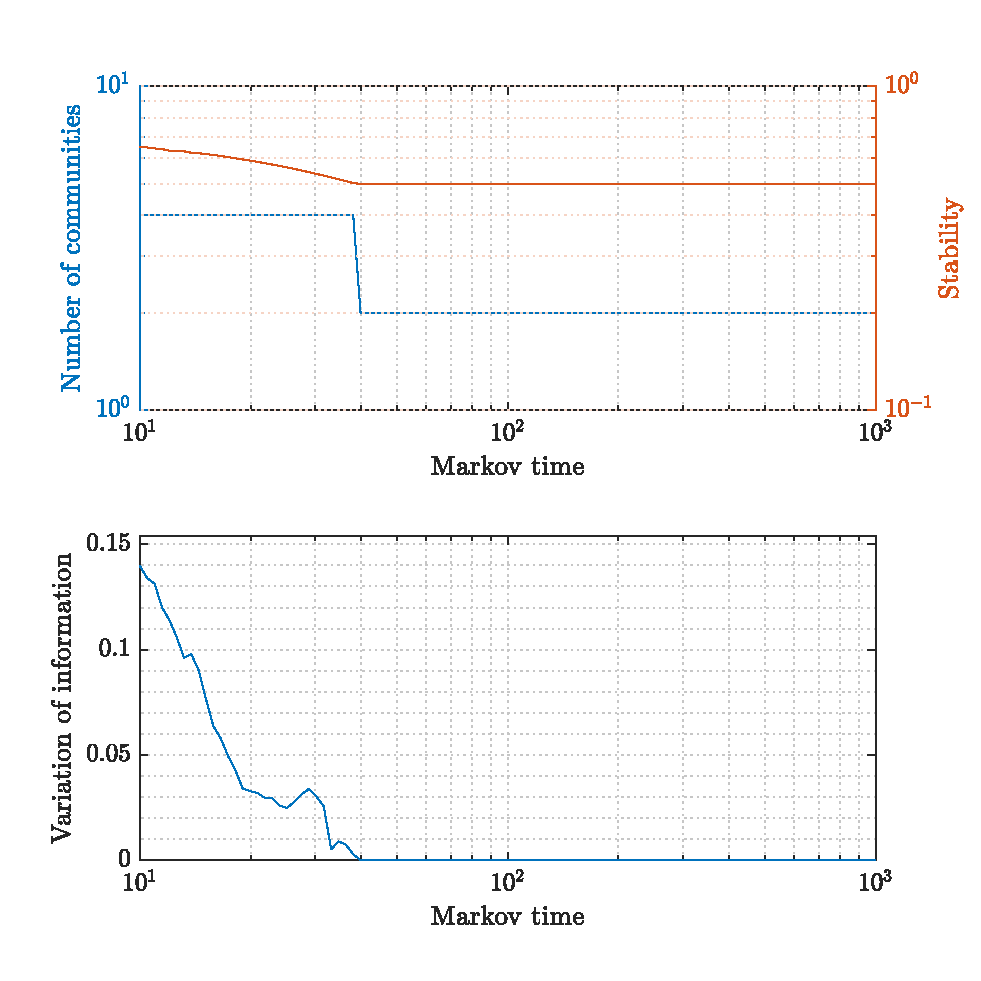
\includegraphics[width = .7\textwidth, height = .4\textheight]{fig/problem2box/stab_a1.eps}
	\caption{Stability, number of communities and variation of information as a function of the Markov time for $\alpha = 1$.}
	\label{fig:staba1}
\end{figure}

\begin{figure}[!htp]
	\centering
	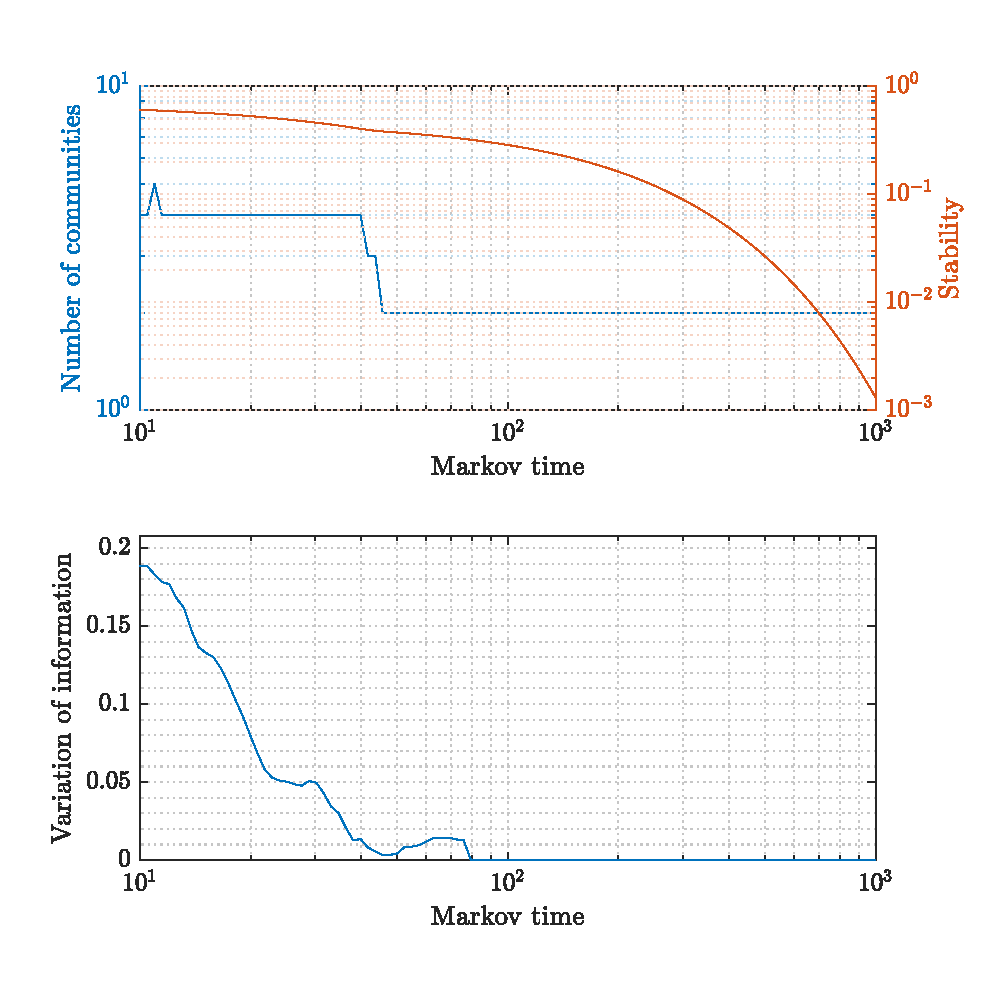
\includegraphics[width = .7\textwidth, height = .4\textheight]{fig/problem2box/stab_a75.eps}
	\caption{Stability, number of communities and variation of information as a function of the Markov time for $\alpha = 0.75$.}
	\label{fig:staba75}
\end{figure}

\begin{figure}[!htp]
	\centering
	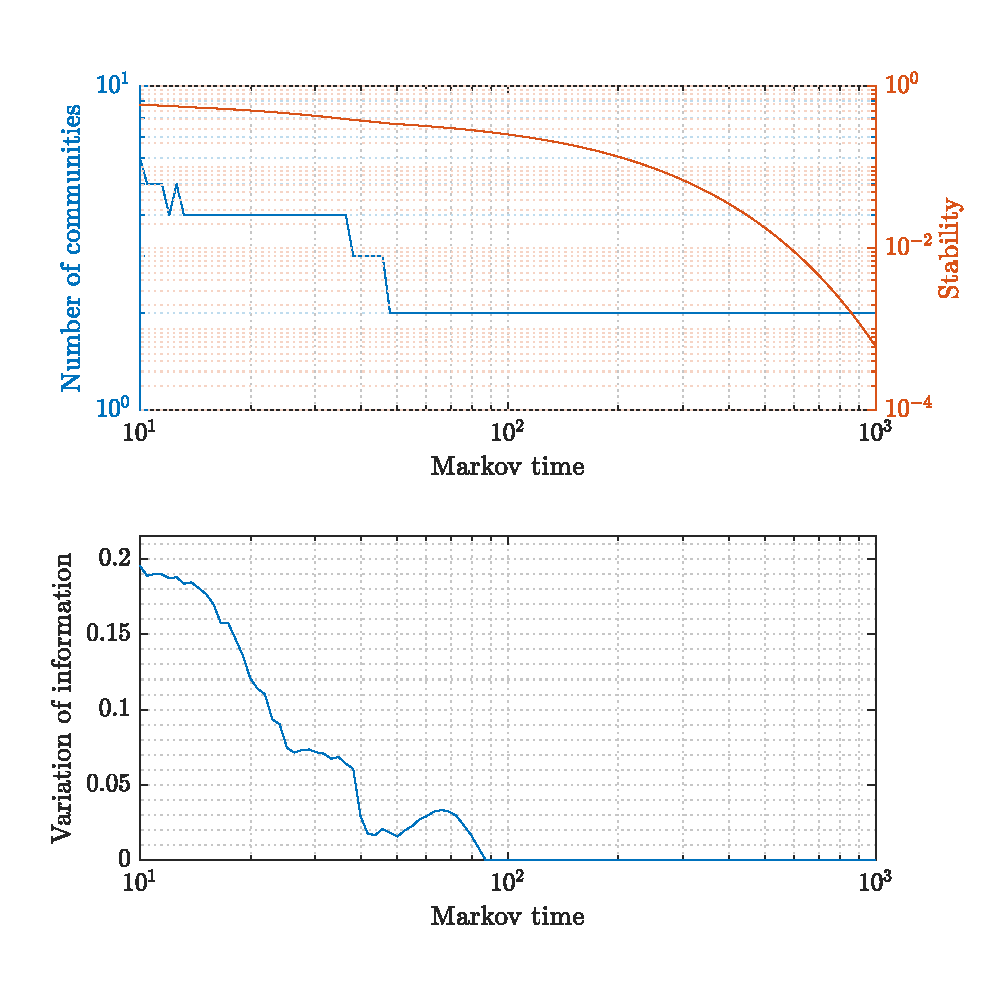
\includegraphics[width = .7\textwidth, height = .4\textheight]{fig/problem2box/stab_a5.eps}
	\caption{Stability, number of communities and variation of information as a function of the Markov time for $\alpha = 0.5$.}
	\label{fig:staba5}
\end{figure}

\begin{figure}[!htp]
	\centering
	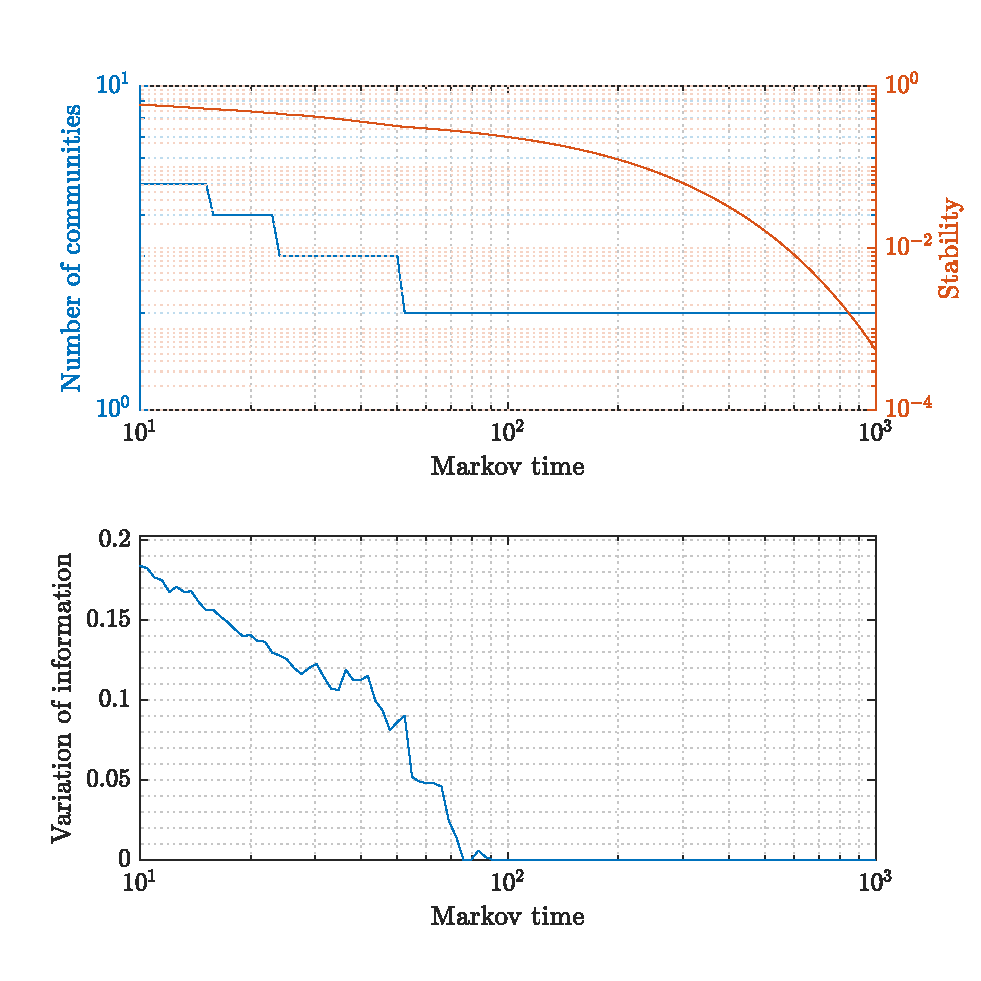
\includegraphics[width = .7\textwidth, height = .4\textheight]{fig/problem2box/stab_a25.eps}
	\caption{Stability, number of communities and variation of information as a function of the Markov time for $\alpha = 0.25$.}
	\label{fig:staba25}
\end{figure}

\begin{figure}[!htp]
	\centering
	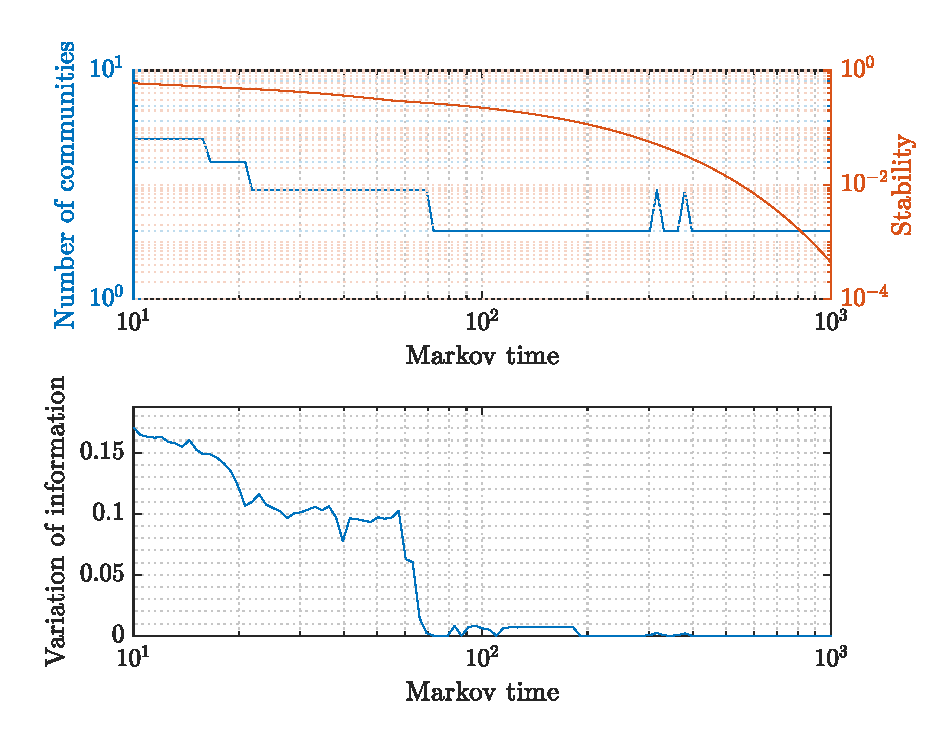
\includegraphics[width = .7\textwidth, height = .4\textheight]{fig/problem2box/stab_a0.eps}
	\caption{Stability, number of communities and variation of information as a function of the Markov time for $\alpha = 0$.}
	\label{fig:staba0}
\end{figure}

\begin{figure}[!htp]
	\centering
	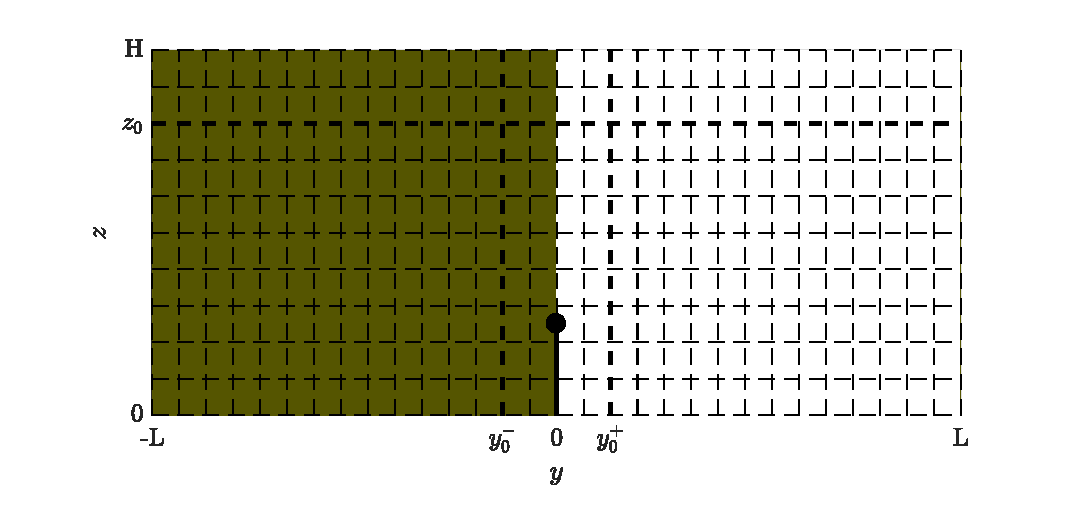
\includegraphics[width = .7\textwidth]{fig/problem2box/cluster_a25_2_.eps}
	\caption{Illustration of the two-communities partitioning for $\alpha = 0.25$.}
	\label{fig:cluster_a25_2}
\end{figure}

\begin{figure}[!htp]
	\centering
	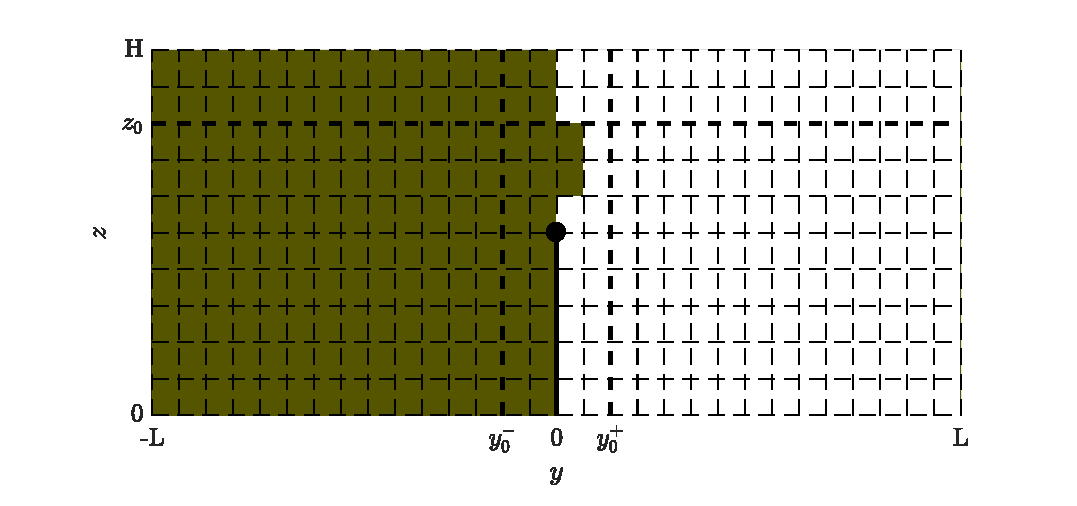
\includegraphics[width = .7\textwidth]{fig/problem2box/cluster_a5_2_.eps}
	\caption{Illustration of the two-communities partitioning for $\alpha = 0.5$.}
	\label{fig:cluster_a5_2}
\end{figure}

\begin{figure}[!htp]
	\centering
	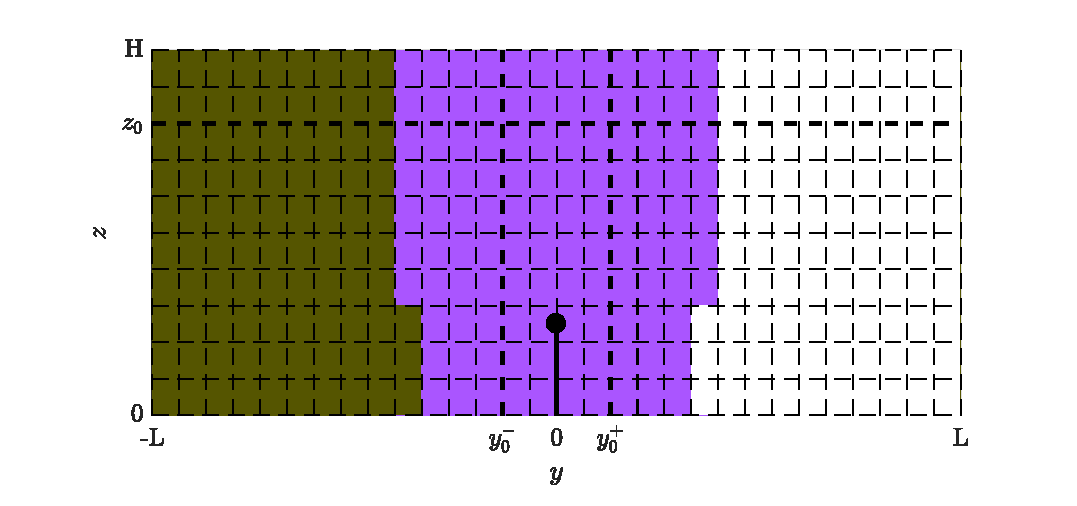
\includegraphics[width = .7\textwidth]{fig/problem2box/cluster_a25_3_.eps}
	\caption{Illustration of the three-communities partitioning for $\alpha = 0.25$.}
	\label{fig:cluster_a25_3}
\end{figure}

\begin{figure}[!htp]
	\centering
	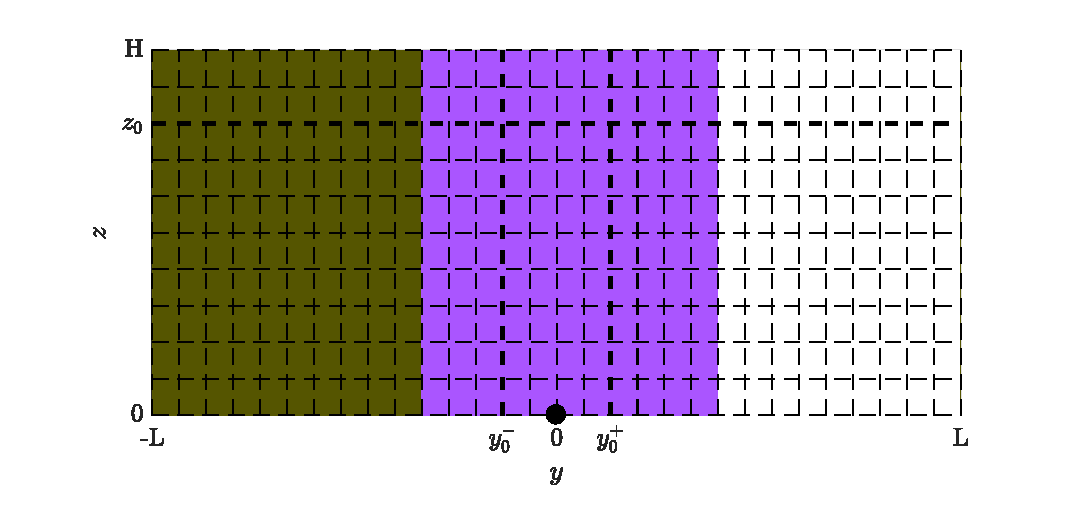
\includegraphics[width = .7\textwidth]{fig/problem2box/cluster_a0_3_.eps}
	\caption{Illustration of the three-communities partitioning for $\alpha = 0$.}
	\label{fig:cluster_a0_3}
\end{figure}

\newpage
\section{Building a compartment model}
Let us now focus on the case $\alpha = 0.75$. The community detection method applied in the previous section suggests a two compartments model with $\Omega_1 = \Omega^-$ and $\Omega_2 = \Omega^+$. We consider a \textit{passive} tracer and the domain is \textit{isolated}. First, in section~\ref{subsec:limitations}, the limitations of such a two-compartment model are discussed \textit{a priori}. Then, two approaches are proposed in order to build a compartment model: in section~\ref{sec:ctcm}, a continuous-time compartment model is build which depends on one parameter, and the analytical solution to that compartment model is used together with a numerical simulation to compute a relevant value for that parameter; in section~\ref{sec:dtcm}, a discrete-time compartment model is build which also depends on one parameter, and a numerical simulation is used to estimate that parameter.  

In this section, $\b c(t) = (C_1(t),C_2(t))$ denotes the vector of the average concentrations over the compartments:
\begin{equation}
	C_i(t) = \frac{1}{|\Omega_i|} \int_{\Omega_i} C(\b x,t) \rm d\Omega_i \quad \mbox{for } i = 1,2,
\end{equation}
where $C(\b x,t)$ denotes the concentration function. Notice that since we consider a passive tracer in an isolated domain, the mean concentration $\bar C(t)$ is constant and
\begin{equation}
	\bar C(t) = \bar C = \frac{|\Omega_1| C_1 + |\Omega_2| C_2}{|\Omega|} = \frac{C_1 + C_2}{2},
\end{equation}
where we have used the fact that $|\Omega_1| = |\Omega_2| = |\Omega|/2$. Hence, we can express $C_2$ as a linear function of $C_1$:
\begin{equation} \label{eq:C2-C1}
	C_2 = 2\bar C - C_1.
\end{equation}
In the next, it will thus be sufficient to analyze only the quantity $C_1$, since the error on $C_2$ is exactly the opposite of the error on $C_1$.


\subsection{Limitations of the compartment model} \label{subsec:limitations}
The main limitation of a compartment model is that it only "sees" the average concentration over compartments. In particular, for a same initial condition $C_1(0)$ to the compartment model, an infinity of tracer repartitions within $\Omega_1$ are possible. In this section, we illustrate three different initial repartitions of the particles leading to the same initial condition $C_1(0)$ and thus to the same function $C_1(t)$ in the compartment model.

A first possible initial repartition of the particles is when the tracer mass is uniformly distributed over $\Omega_1$. We denote that initial condition $C^1(0)$. The second case that we consider is when the particles are uniformly distributed over $[-L,-L/2]\times[0,H]$ and there is no particle in $]-L/2,0[\times[0,H]$; it is denoted $C^2(0)$. The last case is when all the tracer mass is concentrated on a single point, chosen here to be in the lower left corner of the domain (the precise location is $(-\frac{14}{15}L,\frac{1}{10}H)$); it is denoted $C^3(0)$. Those three possible initial repartitions of the particles, all leading to the same compartment initial condition $C_1(0)$ (and thus to the same $C_1(t)$ for all $t \ge 0$), are represented in figure~\ref{fig:CI_init}. 

Let $C_1^i(t)$ denote the aggregated concentration over compartment 1 at time $t$ corresponding to the initial repartition of the particles $C^i(0)$ for $i = 1,2,3$. The evolutions of $C^1_1(t)$, $C^2_1(t)$ and $C^3_1(t)$ over 1000 years are shown in figure~\ref{fig:CI_evol}. The compartment model assumption is that the concentration is approximately uniform over the compartments. Hence, we shall expect the compartment model solution $C_1(t)$ corresponding to the initial condition $C_1(0) = C^1_1(0) = C^2_1(0) = C^3_1(0) = 2\bar C$ to be close to $C^1_1(t)$. As expected, $C_1^1(t)$ starts decreasing immediately, since there are already many particles in the exchange zone at $t=0$. In the two other cases, plateaux are observed. Their lengths correspond to the time for the particles to reach the exchange zone and then possibly enter $\Omega_2$. Obviously, this time is larger in case 3 than in case 2. In both cases, once particles have entered the exchange zone, their concentration in the exchange zone is larger than in case 1, allowing for a larger flux of particles towards $\Omega_2$. Hence, at the end of the plateau, the concentration decreases faster in case 2 than it does initially in case 1 and it decreases still faster in case 3 than in case 2. After 100 years, $C^1_1(t)$ and $C^2_1(t)$ are almost confounded but $C^3_1(t)$ stays clearly different until it reaches equilibrium after approximately 700 years.

The point is that those three cases could never be rendered exactly by a compartment model with two compartments since they correspond exactly to the same compartment solution. Hence, we shall not expect too much from our compartment model: a good compartment model should produce a curve that corresponds approximately to $C_1^1(t)$.
\begin{figure}[!htp]
	\centering
	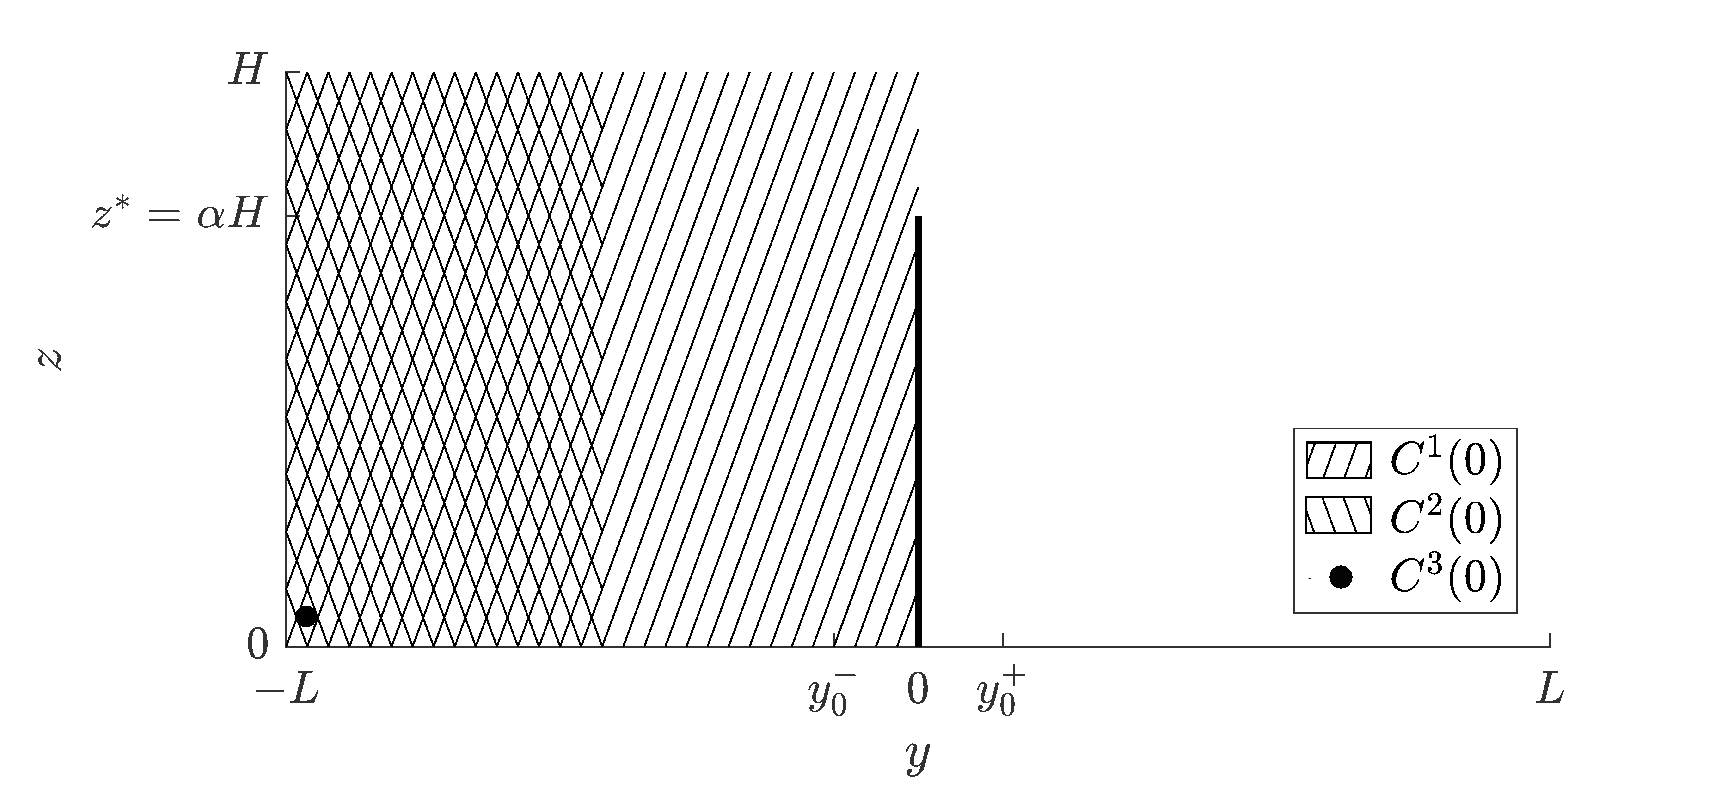
\includegraphics[width = \textwidth]{fig/problem2box/CI_init.eps}
	\caption{Illustration.}
	\label{fig:CI_init}
\end{figure}

\begin{figure}[!htp]
	\centering
	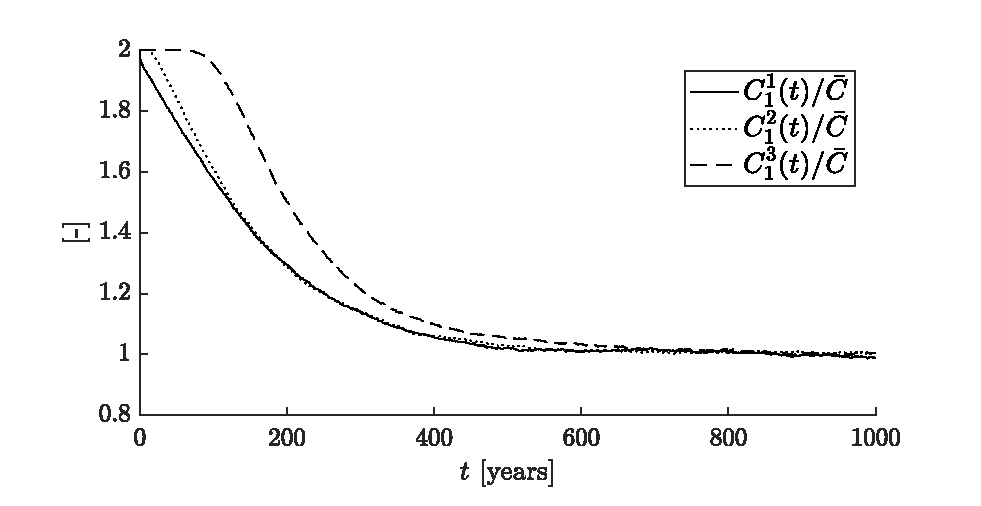
\includegraphics[scale=1]{fig/problem2box/CI_1000years.eps}
	\caption{Comparison of the compartment model solution with the numerical solution for the initial condition $C_1(0) = 2\bar C$.}
	\label{fig:CI_evol}
\end{figure}

\subsection{Continuous-time compartment model} \label{sec:ctcm}
Let $\b A$ be the $2 \times 2$ interaction matrix, and let $\b c$ and $\bs \Omega$ be defined as in~\eqref{eq:def_compartment_vars}. The evolution of the concentration in the two compartments is given by
\begin{equation} \label{eq:generalEDOp2b}
 	\bs \Omega \b{\dot{c}} = \b A \b c.
\end{equation}
It remains to propose an expression for $\b A$. In the general case, a $2 \times 2$ matrix such as $\b A$ has four independent entries. However, properties~\ref{prop1bis_comp}, \ref{prop2bis_comp} and~\ref{prop3bis_comp} shown in chapter~\ref{chap:compartment} imply that $\b A$ has only one degree of freedom. Besides, for $a > 0$, $\b A$ must have the following form:
\begin{equation} \label{eq:A}
	\b A = \begin{pmatrix}
		-a & a\\
		a & -a
	\end{pmatrix}.
\end{equation}
This is nothing but a straightforward implication of the combination of the three properties. Another way of seeing this is by looking at the general form of $\b A$ shown in~\eqref{eq:generalA}. In this case, that expression reduces to (remember that $U_{i,i} = 0 = V_{i,i}$):
\begin{equation} \label{eq:Atemp}
	\b A = \begin{pmatrix}
		-\frac{1}{2} U_{1,2} - V_{1,2} & -\frac{1}{2}U_{1,2} + V_{1,2}\\
		-\frac{1}{2}U_{2,1} + V_{2,1} & -\frac{1}{2}U_{2,1} - V_{2,1}
	\end{pmatrix}.
\end{equation}
By the continuity equation for the compartment model~\eqref{eq:continuitycompartment}, $U_{1,2} = U_{2,1} = 0$, and by the property~\eqref{eq:Vprop} of $V_{i,j}$, $V_{1,2} = V_{2,1} > 0$. With those considerations,~\eqref{eq:Atemp} simplifies to
\begin{equation}
	\b A = \begin{pmatrix}
		- V_{1,2} & V_{1,2}\\
		V_{1,2} & -V_{1,2}
	\end{pmatrix},
\end{equation}
which is exactly~\eqref{eq:A} with $V_{1,2} = a$.

The compartment model considered here has in fact an analytic solution that is relatively easy to compute. Indeed, by~\eqref{eq:C2-C1}, we can express $C_2$ as a linear function of $C_1$ and~\eqref{eq:generalEDOp2b} reduces to a simple ODE in $C_1$ with one parameter $a$:
\begin{equation} \label{eq:edoC1_p2b_a75}
	\frac{dC_1}{dt} = -2aC_1 + 2a\bar C,
\end{equation}
where we have redefined $a$ as $V_{1,2}/|\Omega_1|$ in order to simplify the notations. Let $C_{1,0}$ be the initial condition on $C_1$, namely $C_1(0) = C_{1,0}$. The solution to~\eqref{eq:edoC1_p2b_a75} is easily computed as:
\begin{equation}
	C_1(t) = (C_{1,0} - \bar C) \Exp^{-2at} + \bar C.
\end{equation}
Let us consider the scaled form of the concentration $\tilde C_1 = C_1/\bar C$. The solution is expressed in terms of $\tilde C_1$ as:
\begin{equation}
	\tilde C_1(t) = (\tilde C_{1,0} - 1) \Exp^{-2at} + 1.
\end{equation}

The goal now is to estimate the parameter $a$. To this end, we propose the following approach:
\begin{enumerate}
	\item Run a simulation on a particular instance of the bi-overturner problem (i.e. a particular initial condition).
	\item Using that simulation, compute the average concentration in $\Omega_1$ at $m$ different times $t_0 < t_1 < \dots < t_m$. For the next, let $\bar C_1(t)$ denote the average concentration over $\Omega_1$ at time $t$ (whereas $C_1(t)$ stands for the compartment model concentration in the compartment corresponding to the subdomain $\Omega_1$).
	\item Apply the method of least squares to compute $a$:
	\begin{equation} \label{eq:a_minimization}
		a = \argmin_a \sum_{i=1}^m \left(C_1(t_i)-\bar C_1(t_i)\right)^2.
	\end{equation}
\end{enumerate}
This method leads to a value of $a$ based on one single particular instance of the problem (i.e. a particular initial condition). Of course, we will need to check that the results obtained for other initial conditions are sufficiently close to the simulations.

The method is applied for the initial condition $\tilde C_{1,0} = 2$ (and hence $\tilde C_2(0) = 0$), and with the tracer particles initially uniformly distributed over $\Omega_1$. The simulation is run for 1000 years, and $\bar C_1(t)$ is evaluated every year. The minimization of~\eqref{eq:a_minimization} is performed in \matlab using the Gauss-Newton algorithm, which is well-suited to solve non-linear least squares problems.\footnote{See for example the wikipedia page of the algorithm : \url{https://en.wikipedia.org/wiki/Gauss-Newton_algorithm}.} The value 
\begin{equation}
	a = 0.003125
\end{equation}
is found. Figure~\ref{fig:comparison_comp-real1} compares the evolution of $\tilde C_1(t) = C_1(t)/\bar C$, the analytical solution of the compartment model, with the evolution of $\tilde C_1(t)/\bar C$, the scaled mean value of the concentration over $\Omega_1$ computed numerically, which we may consider as an approximation of the exact solution.

\textcolor{red}{todo : autres conditions initiales}

\subsection{Discrete-time compartment model} \label{sec:dtcm}
When there are more than two compartments, finding an analytic solution is not always possible and the methodology presented in the previous section cannot be applied. For this reason, another approach is proposed in this section. 
\subsubsection{The method}
Here a \textit{discrete} interaction matrix $\b A_{\Delta t}$ is build based on a numerical simulation over a period $\Delta t$. This methodology is thus far more general than the one presented in the previous section. It goes as follows: to compute the entry $[\b A_{\Delta t}]_{i,j}$, run a simulation over a period $\Delta t$, with all the particles initially uniformly distributed over compartment $j$ (i.e. subdomain $\Omega_j$). Let $P_0$ be the total number of particles, and $P_{j \rightarrow i}(\Delta t)$ the number of particles amongst those initially in compartment $j$ that end up in compartment $i$ after a time $\Delta t$. The factor $\frac{P_{j \rightarrow i}(\Delta t)}{P_0}$ is an approximation of the probability to go from compartment $j$ to compartment $i$ within a time period $\Delta t$. But this probability is precisely given by $\frac{|\Omega_i|}{|\Omega_j|}[\b A_{\Delta t}]_{i,j}$, as explained page \pageref{page:probability_interpretation}. We have thus the approximation
\begin{equation} \label{eq:A_approx_discr}
	[\b A_{\Delta t}]_{i,j} \approx \frac{P_{j \rightarrow i}(\Delta t)}{P_0}\frac{|\Omega_j|}{|\Omega_i|}.
\end{equation}
Using that formula to compute an approximation of $\b A_{\Delta t}$, it is seen that properties~\ref{prop1_discr_comp}, \ref{prop2_discr_comp} and~\ref{prop5_discr_comp} are always respected \textit{a priori}. Properties~\ref{prop3_discr_comp} and~\ref{prop4_discr_comp} should by verified a posteriori.
\subsubsection{Results}
In a first instance, we can take advantage of the properties developed in section~\ref{sec:dtcm(chapcomp)} to deduce the general form of $\b A_{\Delta t}$ for this problem. In the present case, $\Omega_1$ and $\Omega_2$ have the same size; this implies that property~\ref{prop2_discr_comp} reduces to corollary~\ref{corollary2}, and that property~\ref{prop5_discr_comp} becomes equivalent to property~\ref{prop4_discr_comp}. Putting everything together, the matrix $\b A_{\Delta t}$ that we search is a $2 \times 2$ matrix whose entries are comprised between 0 and 1 and which satisfies $\b 1^\t \b A_{\Delta t} = \b 1^\t$ and $\b A_{\Delta t} \b 1= \b 1$. This implies that $\b A_{\Delta t}$ must have the following form:
\begin{equation} \label{eq:generalformAdeltat}
	\b A_{\Delta t} = \begin{pmatrix}
		a & 1-a\\ 1-a & a
	\end{pmatrix},
\end{equation}
for some $a \in [0,\,1]$.

The discrete interaction matrix is approximated for $\Delta t = 1$ year with $P_0 = 10\ 000$. \textcolor{red}{Mentionner l'étude de convergence, mais la rendre plus rigoureuse.} Using formula~\eqref{eq:A_approx_discr}, we get
\begin{equation}
	\b A_1 = \begin{pmatrix}
		0.9839 & 0.0159 \\ 
		0.0161 & 0.9841
	\end{pmatrix}.
\end{equation}
This approximation of $\b A_1$ does not exactly match the general form~\eqref{eq:generalformAdeltat}. Hence, we improve that approximation by choosing $a$ as an average:
\begin{equation}
	a = \frac{[\b A_1]_{1,1} + (1-[\b A_1]_{1,2}) + (1 - [\b A_1]_{2,1}) + [\b A_1]_{2,2}}{4} = 0.9840,
\end{equation}
leading to
\begin{equation}
	\b A_1^{discr,1} = \begin{pmatrix}
		0.9840 & 0.0160 \\ 
		0.0160 & 0.9840
	\end{pmatrix},
\end{equation}
which match the general form~\eqref{eq:generalformAdeltat}. For any initial condition, we can now approximate the concentration in both compartments after $T$ years as
\begin{equation}
	\b c^{discr,1}(T) = \left(\b A_1^{discr,1}\right)^T \b c(0).
\end{equation}
The resulting evolution of the concentration in compartment 1 is shown in figure~\ref{fig:comparison_comp-real1} for the initial condition $\b c(0) = (2\bar C,0)^\t$. Clearly, this result is not satisfying as the concentration decreases much too fast in compartment 1. Therefore, we propose another approach: recall from figure~\ref{fig:staba75} that the two-communities clustering is returned by the stability method for times larger than (approximately) 50 years. This suggests that computing the discrete interaction matrix $\b A_{50}$ could provide more interesting results. We get numerically
\begin{equation}
	\b A_{50} = \begin{pmatrix}
		0.8753 &   0.1206\\
	    0.1248  &  0.8795
	\end{pmatrix},
\end{equation}
which is corrected as
\begin{equation}
	\b A_{50} = \begin{pmatrix}
		0.87735 &   0.12265\\
	    0.12265  &  0.87735
	\end{pmatrix}.
\end{equation}
This discrete interaction matrix only allows to compute the concentration at times that are multiples of 50 years. We have the approximation
\begin{equation} \label{eq:cdiscr2}
	\b c^{discr,2}(T) = \left(\b A_{50}\right)^{\frac{T}{50}} \b c(0) \qquad \mbox{for } T = 0,50,100,\dots
\end{equation}
The resulting evolution of the concentration in compartment 1 is also shown in figure~\ref{fig:comparison_comp-real1}. The result is far better than with the first method. Notice that in this case, approximating $\b A_1$ as
\begin{equation}
	\b A_1^{discr,2} = \left(\b A_{50}\right)^{\frac{1}{50}},
\end{equation}
yields
\begin{equation}
	\b A_1^{discr,2} = \begin{pmatrix}
		0.9972 & 0.0028 \\ 
		0.0028 & 0.9972
	\end{pmatrix}.
\end{equation}
The resulting approximation of the concentration is the same as in equation~\eqref{eq:cdiscr2} but now we are able to compute the concentration in the compartments every year. Notice that this does not provide a general method to compute $\b A_1$ since we have no a priori guarantee that the entries of $(\b A_{\Delta t})^{\frac{1}{\Delta t}}$ are real.

This section presents a procedure to numerically estimate the discrete transition matrix $\b A_{\Delta t}$ for any time step $\Delta t$. However, the bad results obtained with our first estimation of $\b A_1$ show that the choice of $\Delta t$ is crucial. Let $[t_a,\, t_b]$ denote the time range at which the clustering chosen to delineate the subdomains is found by the stability method. The results of this section suggest that $\Delta t = t_a$ could be a satisfying choice. Unfortunately, no conclusion can be drawn based only on this simple example, and the method would need to be applied on more complicated problems.

\begin{figure}[!htp]
	\centering
	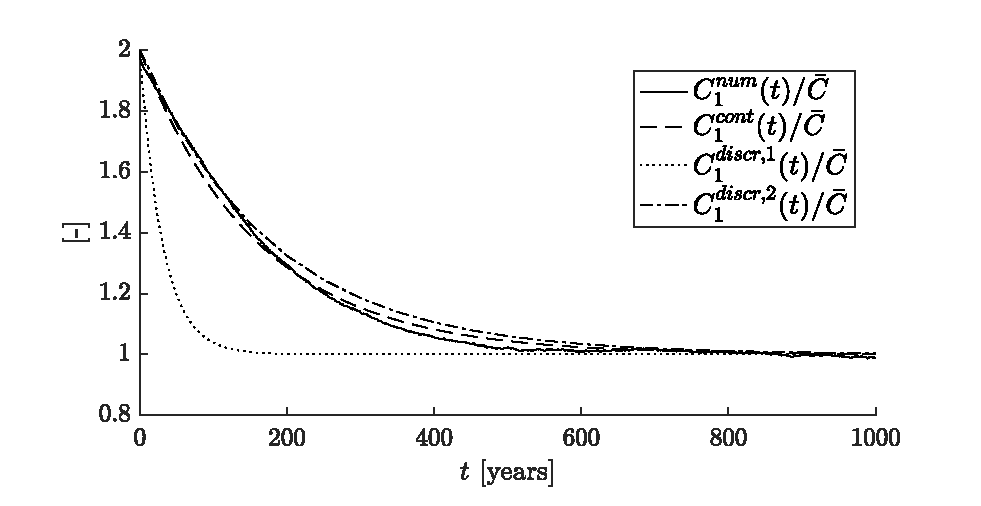
\includegraphics[scale=1]{fig/problem2box/C1vsC1tilde1_1000years2.eps}
	\caption{Comparison of the compartment model solution with the numerical solution for the initial condition $C_1(0) = 2\bar C$.}
	\label{fig:comparison_comp-real1}
\end{figure}